\documentclass[11pt]{book}
\usepackage[paperheight=9in,paperwidth=6in]{geometry}
%\pagenumbering{gobble}
\usepackage{fontspec}
\usepackage{fancyhdr}
\usepackage{graphicx}
%\usepackage{pdfpages}
\usepackage[autocompile]{gregoriotex}
\grechangestyle{abovelinestext}{\normalfont}
\def\GreStar{*}

\setmainfont{EB Garamond}[UprightFont=EB Garamond Regular,
ItalicFont= EB Garamond Italic,
BoldFont= EB Garamond Bold,
Ligatures=Rare,
StylisticSet=6,
Numbers=OldStyle]

\newcommand{\rubrique}[1]{{\fontsize{9}{11}\selectfont\textit{#1}}}
\newcommand{\normaltext}[1]{{\normalfont\fontsize{9}{11}\selectfont{#1}}}

\pagestyle{fancy}
\fancyhead{}
\fancyfoot{}
\renewcommand{\headrulewidth}{0pt}


\fancyhead[RO]{\small\sc\addfontfeature{LetterSpace=3.0}{{Commemorationes Sanctorum}}\hspace{0.5cm}\thepage}
\fancyhead[LE]{\small\thepage\hspace{0.5cm}\sc\addfontfeature{LetterSpace=3.0}{Ad Laudes et Vesperas}}

\newcommand{\setheaders}[2]{
	\renewcommand{\rightmark}{{\sc\addfontfeature{LetterSpace=3.0}#2}}
	\renewcommand{\leftmark}{{\sc\addfontfeature{LetterSpace=3.0}#1}}
}
\setheaders{}{}

\begin{document}
%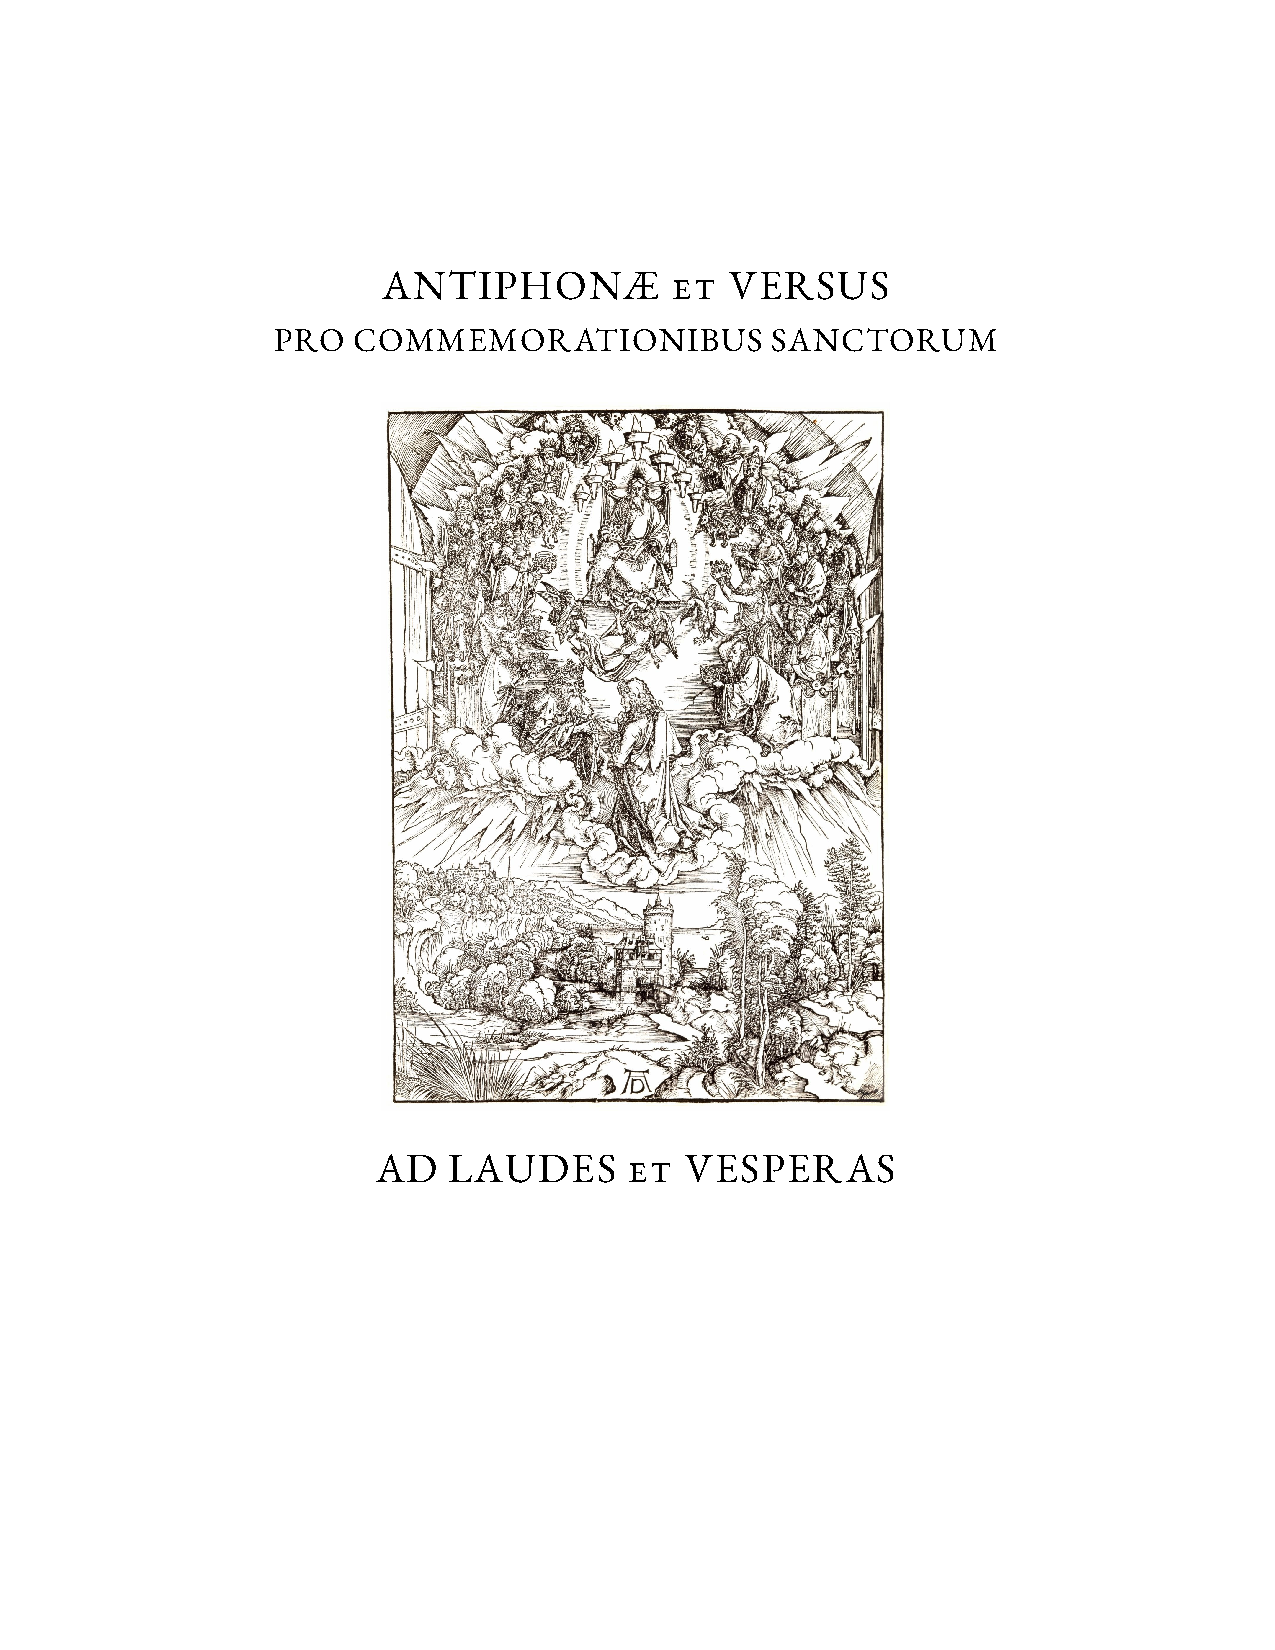
\includepdf[pages=-,noautoscale=true,fitpaper=true]{CommSanctorumCouverture.pdf}
%\begin{titlepage}
% \begin{center}
% \fontsize{20}{25}\selectfont\addfontfeature{LetterSpace=5.0}{ANTIPHONÆ \textsc{et} VERSUS\\ \textsc{pro} COMMEMORATIONIBUS}
% \end{center}
% \vspace{0.4cm}
% \centering
%\includegraphics[width=12cm,height=12cm,keepaspectratio]{Dürer_-_Saint_John_before_God_and_the_Elders}
%\begin{center}
% \fontsize{20}{25}\selectfont\addfontfeature{LetterSpace=5.0}{\textsc{ad} LAUDES \textsc{et} VESPERAS}
% \end{center}
%\end{titlepage}
%\newpage\null\thispagestyle{empty}\newpage

\thispagestyle{empty}
\begin{center}
Pro Martyribus in Tempore Paschalis
\vspace{3mm}

In I Vesperis
\end{center}

\greannotation{Ant.}
\greannotation{1.}
\grechangestyle{initial}{\fontsize{28}{28}\selectfont}
\gregorioscore{Partitions/Lux_perpetua_lucebit}
\vspace{2mm}
\noindent\hspace{3.8mm}℣. Sáncti et jústi in Dómino gaudéte, allelúia.\\
\hspace*{3.8mm}℟. Vos elégiit Déus in hæreditátem síbi, allelúia.

\begin{center}
Ad Laudes
\end{center}

\greannotation{Ant.}
\greannotation{1.}
\grechangestyle{initial}{\fontsize{28}{28}\selectfont}
\gregorioscore{Partitions/Filiae_Jerusalem}
\vspace{2mm}
\noindent\hspace{3.8mm}℣. Pretiósa in conspéctu Dómini, allelúia.\\
\hspace*{3.8mm}℟. Mors sanctórum éjus, allelúia.

\begin{center}
In II Vesperis
\end{center}

\greannotation{Ant.}
\greannotation{1.}
\grechangestyle{initial}{\fontsize{28}{28}\selectfont}
\gregorioscore{Partitions/Sancti_et_justi_in_domino}
\vspace{2mm}
\noindent\hspace{3.8mm}℣. Pretiósa in conspéctu Dómini, allelúia.\\
\hspace*{3.8mm}℟. Mors sanctórum éjus, allelúia.

\rubrique{Si facienda sit commemoratio alterius Officii quod habet eamdem Antiphonam dictitur \normaltext{Ant. Filiæ Jerusalem,  ℣. Pretiósa.} ut supra. Si jam dictus sit, dicitur:}

\noindent\hspace{4.9mm}℣. Lux perpétua lucébit sánctis túis Dómine, allelúia.\\
\hspace*{4.9mm}℟. Et ætérnitas témporum, allelúia.

\begin{center}
Pro Uno Martyre Extra Tempus Paschale
\vspace{3mm}

In I Vesperis
\end{center}

\greannotation{Ant.}
\greannotation{8.}
\grechangestyle{initial}{\fontsize{28}{28}\selectfont}
\gregorioscore{Partitions/Iste_sanctus_pro_lege}
\vspace{2mm}
\noindent\hspace{3.8mm}℣. Glória et honóre coronásti éum Dómine.\\
\hspace*{3.8mm}℟. Et constituísti éum super ópera mánuum tuárum.

\begin{center}
\vspace{-6mm}
Ad Laudes
\end{center}

\greannotation{Ant.}
\greannotation{3.}
\grechangestyle{initial}{\fontsize{28}{28}\selectfont}
\gregorioscore{Partitions/Qui_odit_animam_suam}
\vspace{2mm}
\noindent\hspace{3.7mm}℣. Jústus ut pálma florébit.\\
\hspace*{3.7mm}℟. Sicut cédrus Líbani multiplicábitur.

\begin{center}
In II Vesperis
\end{center}

\greannotation{Ant.}
\greannotation{1.}
\grechangestyle{initial}{\fontsize{28}{28}\selectfont}
\gregorioscore{Partitions/Qui_vult_venire}
\vspace{2mm}
\noindent\hspace{3.7mm}℣. Jústus ut pálma florébit.\\
\hspace*{3.7mm}℟. Sicut cédrus Líbani multiplicábitur.

\rubrique{Si facienda sit commemoratio alterius Martyris quod habet eamdem Antiphonam dictitur \normaltext{Ant. Qui ódit,  ℣. Jústus ut pálma.} ut supra. Si jam dictus sit, dicitur:}

\noindent\hspace{3.6mm}℣. Posuísti Dómine super cáput éjus.\\
\hspace*{3.6mm}℟. Corónam de lápide pretióso.
\newpage
%\vspace{-3mm}
\begin{center}
Pro Pluribus Martyribus Extra Tempus Paschale
\vspace{3mm}

In I Vesperis
\end{center}

\greannotation{Ant.}
\greannotation{8.}
\grechangestyle{initial}{\fontsize{28}{28}\selectfont}
\gregorioscore{Partitions/Istorum_est_enim}
\vspace{2mm}
\noindent\hspace{3.8mm}℣. Lætámini in Dómino et exultáte jústi.\\
\hspace*{3.8mm}℟. Et gloriámini ómnes récti córde.

\begin{center}
Ad Laudes
\end{center}

\greannotation{Ant.}
\greannotation{5.}
\grechangestyle{initial}{\fontsize{28}{28}\selectfont}
\gregorioscore{Partitions/Vestri_capilli_capitis}
\vspace{2mm}
\noindent\hspace{3.7mm}℣. Exsultábunt Sáncti in glória.\\
\hspace*{3.7mm}℟. Lætabúntur in cubílibus súis.

\begin{center}
In II Vesperis
\end{center}

\greannotation{Ant.}
\greannotation{6.}
\grechangestyle{initial}{\fontsize{28}{28}\selectfont}
\gregorioscore{Partitions/Gaudent_in_caelis}
\vspace{2mm}
\noindent\hspace{3.8mm}℣. Exsultábunt Sáncti in glória.\\
\hspace*{3.8mm}℟. Lætabúntur in cubílibus súis.

\rubrique{Si facienda sit commemoratio alterius Officii quod habet eamdem Antiphonam dictitur \normaltext{Ant. Véstri capíli cápitiis,  ℣. Exsultábunt.} ut supra. Si jam dictus sit, dicitur:}

\noindent\hspace{4.5mm}℣. Exsúltent jústi in conspéctu Déi.\\
\hspace*{4.5mm}℟. Et delecténtur in lætítia.\\

\begin{center}
\vspace{-6mm}
Pro Confessore Pontifice
\vspace{3mm}

In I Vesperis
\end{center}

\grechangedim{maxbaroffsettextleft}{0cm}{fixed}
\greannotation{Ant.}
\greannotation{1.}
\grechangestyle{initial}{\fontsize{28}{28}\selectfont}
\gregorioscore{Partitions/Sacerdos_et_pontifex..._ora}
\vspace{2mm}
\noindent\hspace{3.7mm}℣. Amávit éum Dóminus, et ornávit éum. (\textit{T.P.} Alléluia.)\\
\hspace*{3.7mm}℟. Stólam glóriæ indúit éum. (\textit{T.P.} Alléluia.)

\begin{center}
Ad Laudes
\end{center}

\grechangedim{maxbaroffsettextleft}{0.3cm}{scalable}
\greannotation{Ant.}
\greannotation{1.}
\grechangestyle{initial}{\fontsize{28}{28}\selectfont}
\gregorioscore{Partitions/Euge_serve_bone_Conf_pont}
\vspace{2mm}
\noindent\hspace{3.9mm}℣. Jústum dedúxit Dóminus per vías réctas. (\textit{T.P.} Alléluia.)\\
\hspace*{3.9mm}℟. Et osténdi ílli régnum Déi. (\textit{T.P.} Alléluia.)

\begin{center}
In II Vesperis
\end{center}

\grechangedim{maxbaroffsettextleft}{0cm}{fixed}
\greannotation{Ant.}
\greannotation{1.}
\grechangestyle{initial}{\fontsize{28}{28}\selectfont}
\gregorioscore{Partitions/Amavit_eum_dominus}
\vspace{2mm}
\noindent\hspace{3.9mm}℣. Jústum dedúxit Dóminus per vías réctas. (\textit{T.P.} Alléluia.)\\
\hspace*{3.9mm}℟. Et osténdi ílli régnum Déi. (\textit{T.P.} Alléluia.)

\begin{center}
In II Vesperis Pro Summis Pontificibus
\end{center}

\greannotation{Ant.}
\greannotation{1.}
\grechangestyle{initial}{\fontsize{28}{28}\selectfont}
\gregorioscore{Partitions/Dum_esset_summus_pontifex}
\vspace{2mm}
\noindent\hspace{3.9mm}℣. Jústum dedúxit Dóminus per vías réctas. (\textit{T.P.} Alléluia.)\\
\hspace*{3.9mm}℟. Et osténdi ílli régnum Déi. (\textit{T.P.} Alléluia.)

\rubrique{Si facienda sit commemoratio alterius Officii quod habet eamdem Antiphonam dictitur \normaltext{Ant. Euge, ℣. Jústum.} ut supra. Si jam dictus sit, dicitur:}

\noindent\hspace{4.5mm}℣. Elégit éum Dóminus sacerdótem síbi. (\textit{T.P.} Alléluia.)\\
\hspace*{4.5mm}℟. Ad sacrificándum éi hóstiam láudis. (\textit{T.P.} Alléluia.)

\begin{center}
Pro Doctoribus
\vspace{3mm}

In utrisque Vesperis
\end{center}

\greannotation{Ant.}
\greannotation{2.}
\grechangestyle{initial}{\fontsize{28}{28}\selectfont}
\gregorioscore{Partitions/O_doctor_optime}

\begin{center}
Nomina Doctorum Ecclesiæ
\end{center}

\greseteolcustos{manual}
\gresetinitiallines{0}
\gregorioscore{Partitions/O_doctor_optime_Beda}
\hspace*{-3mm}Ephraem \hspace{8.7mm}Ambró-\hspace{0.6mm}si \hspace{12mm}Cy-\hspace{1.4mm}ríl-\hspace{0.6mm}le \hspace{12.1mm}Hi-\hspace{1mm}lá-\hspace{1.1mm}ri\\
\hspace*{3mm}Lé-\hspace{1.5mm}o \hspace{13.5mm}An-\hspace{0.2mm}sél-\hspace{0.5mm}me \hspace{10.5mm}Francí-sce \hspace{13.5mm}Jo-\hspace{1.3mm}ánnes\\
\hspace*{2.95mm}Pétre \hspace{13mm}Bá-\hspace{2mm}sí-\hspace{4mm}li\\
\hspace*{-0.3mm}Thóma \hspace{12mm}Ro-\hspace{1.2mm}bér-\hspace{1.1mm}te

\gregorioscore{Partitions/O_doctor_optime_Athanasi}
\hspace*{-1.5mm}Augustí-ne\\
\hspace*{5.5mm}I-\hspace{2mm}si-dó-re

\gregorioscore{Partitions/O_doctor_optime_Petre}
\vspace{2mm}
\begin{center}
In I Vesperis
\end{center}
\noindent\hspace*{3.6mm}℣. Amávit éum Dóminus, et ornávit éum. (\textit{T.P.} Alléluia.)\\
\hspace*{3.6mm}℟. Stólam glóriæ indúit éum. (\textit{T.P.} Alléluia.)

\begin{center}
In II Vesperis
\end{center}

\noindent\hspace{3.6mm}℣. Jústum dedúxit Dóminus per vías réctas. (\textit{T.P.} Alléluia.)\\
\hspace*{3.6mm}℟. Et osténdi ílli régnum Déi. (\textit{T.P.} Alléluia.)

\begin{center}
Ad Laudes
\end{center}

\rubrique{Ant. et ℣. de Confessore Pontifice vel non Pontifice, pro qualitate Sancti.}

\begin{center}
Pro Confessore non Pontifice
\vspace{3mm}

In I Vesperis
\end{center}

\greseteolcustos{auto}
\grechangedim{maxbaroffsettextleft}{0cm}{fixed}
\gresetinitiallines{1}
\greannotation{Ant.}
\greannotation{1.}
\grechangestyle{initial}{\fontsize{28}{28}\selectfont}
\gregorioscore{Partitions/Similabo_eum}
\vspace{2mm}
\noindent\hspace{3.6mm}℣. Amávit éum Dóminus, et ornávit éum. (\textit{T.P.} Alléluia.)\\
\hspace*{3.6mm}℟. Stólam glóriæ indúit éum. (\textit{T.P.} Alléluia.)

\begin{center}
Ad Laudes
\end{center}

\grechangedim{maxbaroffsettextleft}{0.3cm}{scalable}
\greannotation{Ant.}
\greannotation{4.}
\grechangestyle{initial}{\fontsize{28}{28}\selectfont}
\gregorioscore{Partitions/Euge_serve_bone_Conf_non_pont}
\vspace{2mm}
\noindent\hspace{4.4mm}℣. Jústum dedúxit Dóminus per vías réctas. (\textit{T.P.} Alléluia.)\\
\hspace*{4.4mm}℟. Et osténdi ílli régnum Déi. (\textit{T.P.} Alléluia.)

\begin{center}
In II Vesperis
\end{center}

\grechangedim{maxbaroffsettextright}{0cm}{fixed}
\greannotation{Ant.}
\greannotation{8.}
\grechangestyle{initial}{\fontsize{28}{28}\selectfont}
\gregorioscore{Partitions/Hic_vir_despiciens}
\vspace{2mm}
\noindent\hspace{3.6mm}℣. Jústum dedúxit Dóminus per vías réctas. (\textit{T.P.} Alléluia.)\\
\hspace*{3.6mm}℟. Et osténdi ílli régnum Déi. (\textit{T.P.} Alléluia.)

\rubrique{Si facienda sit commemoratio alterius Officii quod habet eamdem Antiphonam dictitur \normaltext{Ant. Euge,  ℣. Jústum.} ut supra. Si jam dictus sit, dicitur:}

\noindent\hspace{3.9mm}℣. Os jústi meditábiitur sapiéntiam. (\textit{T.P.} Alléluia.)\\
\hspace*{3.9mm}℟. Et língua éjus loquétur judícium. (\textit{T.P.} Alléluia.)

\begin{center}
Pro  Una Virgine
\vspace{3mm}

In I Vesperis
\end{center}

\greannotation{Ant.}
\greannotation{8.}
\grechangestyle{initial}{\fontsize{28}{28}\selectfont}
\gregorioscore{Partitions/Veni_sponsa_I_Vesp}
\vspace{2mm}
\noindent\hspace{3.6mm}℣. Spécie túa et pulchritúdine túa. (\textit{T.P.} Alléluia.)\\
\hspace*{3.6mm}℟. Inténde próspere procéde, et régna.  (\textit{T.P.} Alléluia.)

\begin{center}
Ad Laudes
\end{center}

\textit{Ant.} Simile est.\\
℣. Diffúsa est grátia in lábiis túis. (\textit{T.P.} Alléluia.)\\
℟. Proptérea bendíxit te Déus in ætérnum. (\textit{T.P.} Alléluia.)

\begin{center}
In II Vesperis
\end{center}

\greannotation{Ant.}
\greannotation{7.}
\grechangestyle{initial}{\fontsize{28}{28}\selectfont}
\gregorioscore{Partitions/Veni_sponsa_II_Vesp}
\vspace{2mm}
\noindent\hspace{3.6mm}℣. Diffúsa est grátia in lábiis túis. (\textit{T.P.} Alléluia.)\\
\hspace*{3.6mm}℟. Proptérea bendíxit te Déus in ætérnum. (\textit{T.P.} Alléluia.)

\begin{center}
Pro  Pluribus Virginibus
\vspace{3mm}

Ad Laudes et ad Vesperas
\end{center}

\greannotation{Ant.}
\greannotation{4.}
\grechangestyle{initial}{\fontsize{28}{28}\selectfont}
\gregorioscore{Partitions/Prudentes_virgines}
\vspace{2mm}
\noindent\hspace{3.7mm}℣. Adducéntur. régi vírgines post éam. (\textit{T.P.} Alléluia.)\\
\hspace*{3.7mm}℟.  Próximæ éjus afferéntur tíbi. (\textit{T.P.} Alléluia.)

\begin{center}
Pro  Una Martyre non Virgine et Una vel Pluribus\\nec Martyribus nec Virginibus
\vspace{3mm}

In I Vesperis
\end{center}

\greannotation{Ant.}
\greannotation{8.}
\grechangestyle{initial}{\fontsize{28}{28}\selectfont}
\gregorioscore{Partitions/Simile_est..._negotiatori}
\vspace{2mm}
\noindent\hspace{3.6mm}℣. Spécie túa et pulchritúdine túa. (\textit{T.P.} Alléluia.)\\
\hspace*{3.6mm}℟. Inténde próspere procéde, et régna.  (\textit{T.P.} Alléluia.)

\begin{center}
Ad Laudes
\end{center}

\greannotation{Ant.}
\greannotation{7.}
\grechangestyle{initial}{\fontsize{28}{28}\selectfont}
\gregorioscore{Partitions/Date_ei_de_fructu}
\vspace{2mm}
\noindent\hspace{3.6mm}℣. Diffúsa est grátia in lábiis túis. (\textit{T.P.} Alléluia.)\\
\hspace*{3.6mm}℟. Proptérea bendíxit te Déus in ætérnum. (\textit{T.P.} Alléluia.)

\begin{center}
In II Vesperis
\end{center}

\greannotation{Ant.}
\greannotation{8.}
\grechangestyle{initial}{\fontsize{28}{28}\selectfont}
\gregorioscore{Partitions/Manum_suam_aperuit}
\vspace{2mm}
\noindent\hspace{3.6mm}℣. Diffúsa est grátia in lábiis túis. (\textit{T.P.} Alléluia.)\\
\hspace*{3.6mm}℟. Proptérea bendíxit te Déus in ætérnum. (\textit{T.P.} Alléluia.)

\begin{center}
Pro  Pluribus Martyribus non Virginibus
%\vspace{3mm}

Ad Laudes et Vesperas
\end{center}

\greannotation{Ant.}
\greannotation{8.}
\grechangestyle{initial}{\fontsize{28}{28}\selectfont}
\gregorioscore{Partitions/Istarum_est_enim}
\vspace{2mm}
\noindent\hspace{4mm}℣. Glória et honóre coronásti éum Dómine. (\textit{T.P.} Alléluia.)\\
\hspace*{3.4mm} ℟. Et constituísti éas super ópera mánuum tuárum. (\textit{T.P.} Alléluia.)


\enddocument